%!TEX root = ./ERL Industrial Robots.tex


%--------------------------------------------------------------------
%--------------------------------------------------------------------
\subsection{Task \emph{Plate Drilling}}
\label{ssec:TaskPlateDrilling}



This task simulates handling of an incomplete or faulty parts from an external component supplier. The factory has to quickly react on such issues and create a process to correct the faulty parts.

%--------------------------------------------------------------------
\subsubsection{Task Description}
\label{sssec:TaskPlateDrillingDescription}
The robot has to pick up incoming cover plates and process each cover plate based on its type accordingly.
The robot performs the task with two networked devices in the factory.
The first networked device is the triggered conveyor belt or TCB which is a composite of the quality control camera and the conveyor belt (see Figure \ref{fig:coverPlateQCC}).
The TCB is responsible for delivering the cover plate (by operating the conveyor belt) and detecting the type of the cover plate being delivered.
The second networked device is the drilling machine (see Figure \ref{fig:coverPlateDrillingMachine}) which is operated by the robot to drill a cone sink to the faulty cover plate.

The cover plate of the bearing box has eight holes for connecting the motor with the bearing box and the four central holes need to have a cone sink (see Figure \ref{fig:coverPlatePerfect}). 
There are two possible defects of a cover plate which need to be accommodated in this task.
The first case is where the supplier forgot to drill one of the cone sinks, which results in a faulty cover plate (see Figure \ref{fig:coverPlateFaulty}). 
The faulty cover plates can be corrected by drilling the cone sink with the drilling machine available in the factory.
The second case is where the cover plate is unusable (see Figure \ref{fig:coverPlateUnusable}) and needs to be returned to the supplier for replacement.\\

\begin{figure}[htb]
  \begin{center}
  	\hfill
	  \subfigure[Perfect]{
		  \scalebox{1.0}[1.0]{
  		  \includegraphics[height=30mm,angle=0,trim=0px 0px 0px 0px,clip]
	  		{./fig/workObjects/cover_plate_perfect.jpg}
			}
		  \label{fig:coverPlatePerfect}
		}
		\hfill
	  \subfigure[Faulty]{
		  \scalebox{1.0}[1.0]{
  		  \includegraphics[height=30mm,angle=0,trim=0px 0px 0px 0px,clip]
	  		{./fig/workObjects/cover_plate_faulty.jpg}
			}
		   \label{fig:coverPlateFaulty}
		}
		\hfill
		 \subfigure[Unusable]{
		  \scalebox{1.0}[1.0]{
  		  \includegraphics[height=30mm,angle=0,trim=0px 0px 0px 0px,clip]
	  		{./fig/workObjects/cover_plate_unusable.jpg}
			}
			\label{fig:coverPlateUnusable}
		}
		\hfill\mbox{}
	  \caption{Three possible states of the cover plate}
  	\label{fig:coverPlateStates} 
	\end{center}
\end{figure}


\begin{figure}[htb]
  \begin{center}
  	\hfill
	  \subfigure[Drilling machine]{
		  \scalebox{1.0}[1.0]{
  		  \includegraphics[height=45mm,angle=90,trim=0px 0px 0px 0px,clip]
	  		{pics/atwork/networked_devices/drillingMachine.jpg}
			}
		   \label{fig:coverPlateDrillingMachine}
		}
		\hfill
		 \subfigure[Quality control camera]{
		  \scalebox{1.0}[1.0]{
  		  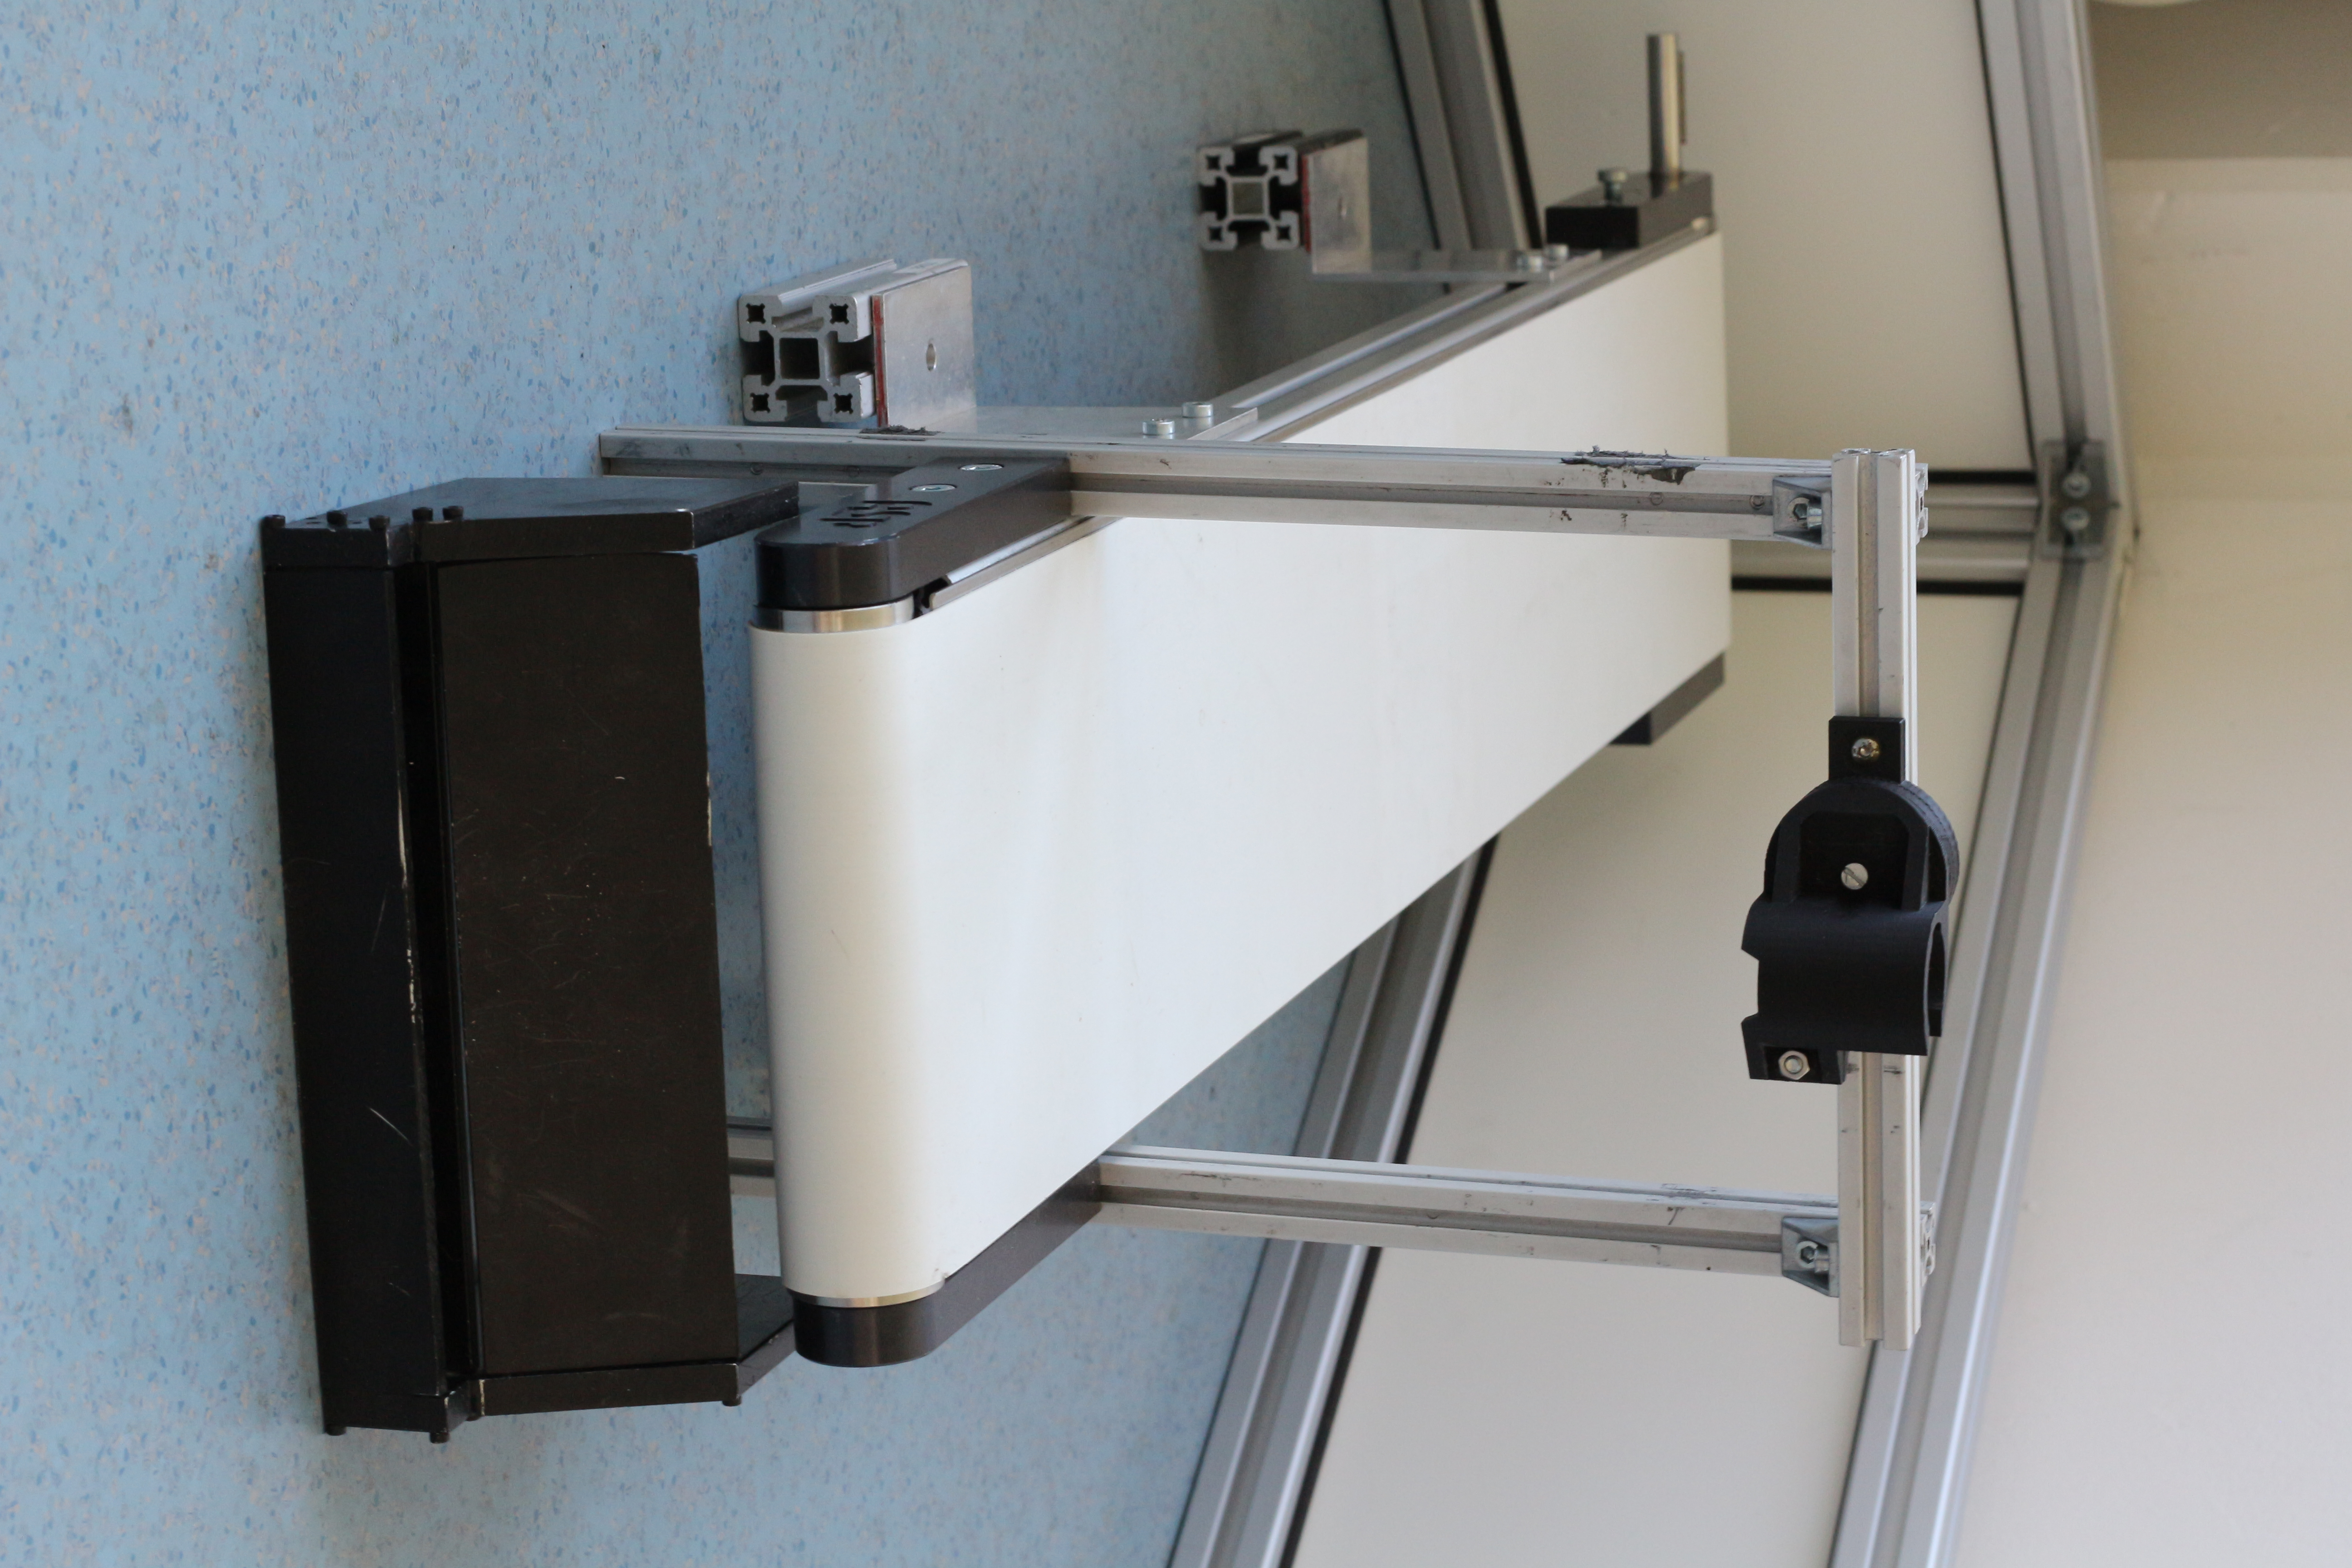
\includegraphics[height=45mm,angle=90,trim=0px 0px 0px 0px,clip]
	  		{pics/atwork/networked_devices/QCC.jpg}
			}
			\label{fig:coverPlateQCC}
		}
		\hfill\mbox{}
	  \caption{Networked devices for the plate drilling task}
  	\label{fig:plateDrillingNetworkedDevices} 
	\end{center}
\end{figure}


%--------------------------------------------------------------------
\subsubsection{Feature Variation}
\label{sssec:TaskPlateDrillingVariation}


The task can have different variations as shown in the following examples.
\begin{itemize}
 \item The sequence of faulty, unusable and perfect plates flowing through the conveyor belt.
 \item The cover plate orientation on the conveyor belt.
 \item The number of plates delivered in each category (faulty, unusable and perfect).
\end{itemize}
Furthermore, the solutions can vary depending on the sequence of activities being performed by the robot. The robot can choose to:

\begin{itemize}
	\item collect all cover plates from the conveyor belt first and process them collectively or
	\item perform the task for one cover plate at a time before collecting the next cover plate from the conveyor belt
\end{itemize}


%--------------------------------------------------------------------
\subsubsection{Input Provided}
\label{sssec:TaskPlateDrillingInput}
The team will be provided with the following information:
\begin{itemize}
\item 3D CAD textured models of the plates
\item Description of three different states of the plate (faulty, unusable, perfect). 
The three different states of the cover plate are shown in Figure \ref{fig:coverPlateStates}.
\item Location of objects related to the task.
\end{itemize}

%--------------------------------------------------------------------
\subsubsection{Expected Robot Behavior or Output}
\label{sssec:TaskPlateDrillingOutput}
The robot operates the conveyor belt and receive the incoming cover plates. 
The robot will fix the faulty cover plates with the drilling machine and deliver the unusable cover plates to trash container box.
The robot has the option to receive and process the plates collectively or individually.

\begin{figure}[htb]
  \begin{center}
  	\hfill
	  \subfigure[Trash container box]{
		  \scalebox{1.0}[1.0]{
  		  \includegraphics[height=35mm,angle=0,trim=0px 0px 0px 0px,clip]
	  		{./fig/Blue_box.jpg}
			}
		   \label{fig:coverPlateUnusableContainerBox}
		}
		\hfill
		 \subfigure[Cover plate file card box]{
		  \scalebox{1.0}[1.0]{
  		  \includegraphics[height=35mm,angle=0,trim=0px 0px 0px 0px,clip]
	  		{pics/atwork/objects/coverPlatesFileBox.jpg}
			}
			\label{fig:coverPlatesFileBox}
		}%
		\hfill\mbox{}
	  \caption{Designated storage for each cover plate type.}
  	\label{fig:coverPlateStorage} 
	\end{center}
\end{figure}

%--------------------------------------------------------------------
\subsubsection{Procedures and Rules}
\label{sssec:TaskPlateDrillingProcedures}
 \begin{description}
     \item [Step 1] The robot commands the TCB to provide a cover plate in the conveyor belt's exit ramp and waits for the result of the plate recognition from CFH.
     \item [Step 2] The robot should pick up the cover plate and either:
	     \begin{itemize}
	     	\item proceed with processing the cover plate received as described in [Step 3] or
	     	\item request for another cover plate as described in [Step 1]
	     	\end{itemize}
     \item [Step 3] There are two possible sequence of actions that need to be executed by the robot depending on the type of the cover plate. If the cover plate is faulty, the robot needs to deliver this to the trash container box. If the cover plate is unusable, the robot needs to:
     	\begin{itemize}
     		\item place the cover plate inside the drilling machine
     		\item perform correction of the cover plate with the drilling machine
     		\item place the corrected cover plate in the file card box.
     	\end{itemize}
\end{description} 

\subsubsection{Communication with CFH}
\label{sssec:CommCFHPlateDrilling}

The communication and interaction between the robot and the networked device is as follows:

\begin{itemize}
	\item \textbf{Triggered conveyor belt} or \textbf{TCB}. This TCB is a composite of the quality control camera and the conveyor belt. The operation of the TCB involves the message types TriggeredConveyorBeltCommand \cite{rockin:CFHMessages}, TriggeredConveyorBeltStatus \cite{rockin:CFHMessages} and Inventory \cite{rockin:CFHMessages}.
For each TriggeredConveyorBeltCommand::START command and \emph{next cycle id} received, the TCB will run the conveyor belt until a cover plate has been recognized and placed in the conveyor belt exit ramp and stop the belt again. 

The \emph{next cycle id} is used to determine the cycle for which the command is executed. It must be exactly one greater than the cycle received via the TriggeredConveyorBeltStatus (next\_cycle = cycle + 1). The cycle determines how often the TCB has already been activated. Every time that the TCB is commanded by a robot, the cycle counter is increased.

The TCB provides information on the type of cover plate (\emph{faulty} or \emph{unusable}) by updating the inventory of the CFH.
	\item \textbf{Drilling machine}. The operation of the drilling machine involves message type DrillingMachineCommand \cite{rockin:CFHMessages} and DrillingMachineStatus \cite{rockin:CFHMessages}
	The drill of the drilling machine will spin continuously and the robot needs to command the drill to move down and up (message of type DrillingMachineCommand \cite{rockin:CFHMessages}). 
	In order to move down the drill, the variable command needs to be set to Command::MOVE\_DOWN. 
	To move the drill up again the variable needs to be set to Command::MOVE\_UP.
	An example in C++ is provided \cite{rockin:CFHExamples}. 
	Additionally, the CFH sends a status message of type DrillingMachineStatus \cite{rockin:CFHMessages} indicating whether the drill is at the top position (state is equal to State::AT\_TOP), at the bottom position (state is equal to State::AT\_BOTTOM), moving down (state is equal to State::MOVING\_DOWN) or moving up (state is equal to State::MOVING\_UP). In case of a problem, the state is equal to State::UNKNOWN.
\end{itemize}

%--------------------------------------------------------------------
\subsubsection{Acquisition of Benchmarking Data}
\label{sssec:TaskPlateDrillingData}

General information on the acquisition of benchmarking data is described in Section \ref{sec:TbmAcquisitionOfData}.

\paragraph{Online Data} In order to send online benchmarking data to the CFH, the robot has to use the \textbf{BenchmarkFeedback} message. The message contains:
\begin{itemize}
	\item after\_receiving (type: PlateState) 
	\item after\_drilling (type: PlateState) 
\end{itemize}

The \textbf{BenchmarkFeedback} message can be found at \cite{rockin:CFHMessages}.

\paragraph{Offline data} 
The additional information described in the following table has to be logged:

\begin{table}[h]
	\centering
	\begin{footnotesize}
		\begin{tabular}{|l|l|l|l|}
			\hline
			Topic	&	Type		&	Frame Id		&	Notes \\ \hline\hline
			/rockin/drill\_command\tablefootnote{Drilling commands issued by the robot} & std\_msgs/Int32 & -- & when issued \\ \hline
			/rockin/qcc\_command\tablefootnote{QCC commands issued by the robot} & std\_msgs/Int32 & -- & when issued \\ \hline
			/rockin/plate\_condition\tablefootnote{Condition of each plate, as evaluated by the robot, after drilling} & std\_msgs/Int32 & -- & when issued \\ \hline
		\end{tabular}
	\end{footnotesize}
\end{table}

%--------------------------------------------------------------------
\subsubsection{Scoring and Ranking}
\label{sssec:TaskPlateDrillingScoring}

Evaluation of the performance of a robot according to this task benchmark is based on performance equivalence classes. Classes are defined in dependence to:
\begin{enumerate}
\item the number and percentage of correctly processed faulty cover plates;
\item the number and percentage of correctly processed unusable cover plates;
\item execution time (if less than the maximum allowed for the benchmark).
\end{enumerate}

\noindent 
\paragraph{Achievements} The set $A$ of achievements for this task includes:
\begin{itemize}
\item the robot communicates with the CFH throughout the test;
\item the team submits the benchmarking data appropriately by the end of the test;
\item the robot picks up a cover plate from the conveyor belt's exit ramp;
\item the robot places an unusable cover plate into the trash container box;
\item the robot completely processes an unusable cover plate (pick up an unusable cover plate from the exit ramp of the conveyor belt and place it into the trash container box);
\item the robot places a faulty cover plates inside the drilling machine;
\item the robot performs the drilling of a faulty cover plate using the drilling machine;
\item the robot completely corrects a faulty cover plate (pick up a faulty cover plate from the exit ramp of the conveyor belt, place it inside the drilling machine and operate the drilling machine);
\item the robot picks up a corrected cover plate from the drilling machine;
\item the robot places a corrected cover plate into the file card box;
\item the robot completely delivers a corrected cover plate (pick up a corrected cover plate from the drilling machine and place it inside the file card box).
\end{itemize}

%--------------------------------------------------------------------
% EOF
%--------------------------------------------------------------------
